\documentclass[]{article}
\usepackage{lmodern}
\usepackage{amssymb,amsmath}
\usepackage{ifxetex,ifluatex}
\usepackage{fixltx2e} % provides \textsubscript
\ifnum 0\ifxetex 1\fi\ifluatex 1\fi=0 % if pdftex
  \usepackage[T1]{fontenc}
  \usepackage[utf8]{inputenc}
\else % if luatex or xelatex
  \ifxetex
    \usepackage{mathspec}
  \else
    \usepackage{fontspec}
  \fi
  \defaultfontfeatures{Ligatures=TeX,Scale=MatchLowercase}
\fi
% use upquote if available, for straight quotes in verbatim environments
\IfFileExists{upquote.sty}{\usepackage{upquote}}{}
% use microtype if available
\IfFileExists{microtype.sty}{%
\usepackage{microtype}
\UseMicrotypeSet[protrusion]{basicmath} % disable protrusion for tt fonts
}{}
\usepackage[margin=1in]{geometry}
\usepackage{hyperref}
\hypersetup{unicode=true,
            pdftitle={Data Visualization in R},
            pdfauthor={Therese Anders},
            pdfborder={0 0 0},
            breaklinks=true}
\urlstyle{same}  % don't use monospace font for urls
\usepackage{graphicx,grffile}
\makeatletter
\def\maxwidth{\ifdim\Gin@nat@width>\linewidth\linewidth\else\Gin@nat@width\fi}
\def\maxheight{\ifdim\Gin@nat@height>\textheight\textheight\else\Gin@nat@height\fi}
\makeatother
% Scale images if necessary, so that they will not overflow the page
% margins by default, and it is still possible to overwrite the defaults
% using explicit options in \includegraphics[width, height, ...]{}
\setkeys{Gin}{width=\maxwidth,height=\maxheight,keepaspectratio}
\IfFileExists{parskip.sty}{%
\usepackage{parskip}
}{% else
\setlength{\parindent}{0pt}
\setlength{\parskip}{6pt plus 2pt minus 1pt}
}
\setlength{\emergencystretch}{3em}  % prevent overfull lines
\providecommand{\tightlist}{%
  \setlength{\itemsep}{0pt}\setlength{\parskip}{0pt}}
\setcounter{secnumdepth}{0}
% Redefines (sub)paragraphs to behave more like sections
\ifx\paragraph\undefined\else
\let\oldparagraph\paragraph
\renewcommand{\paragraph}[1]{\oldparagraph{#1}\mbox{}}
\fi
\ifx\subparagraph\undefined\else
\let\oldsubparagraph\subparagraph
\renewcommand{\subparagraph}[1]{\oldsubparagraph{#1}\mbox{}}
\fi

%%% Use protect on footnotes to avoid problems with footnotes in titles
\let\rmarkdownfootnote\footnote%
\def\footnote{\protect\rmarkdownfootnote}

%%% Change title format to be more compact
\usepackage{titling}

% Create subtitle command for use in maketitle
\newcommand{\subtitle}[1]{
  \posttitle{
    \begin{center}\large#1\end{center}
    }
}

\setlength{\droptitle}{-2em}

  \title{Data Visualization in \texttt{R}}
    \pretitle{\vspace{\droptitle}\centering\huge}
  \posttitle{\par}
  \subtitle{FSU Summer Methods School, Day 1}
  \author{Therese Anders}
    \preauthor{\centering\large\emph}
  \postauthor{\par}
      \predate{\centering\large\emph}
  \postdate{\par}
    \date{5/6/2019}


\begin{document}
\maketitle

\hypertarget{roadmap-for-this-workshop}{%
\section{Roadmap for this workshop}\label{roadmap-for-this-workshop}}

\hypertarget{day-1-basics-of-data-visualization}{%
\subsection{Day 1: Basics of data
visualization}\label{day-1-basics-of-data-visualization}}

\begin{enumerate}
\def\labelenumi{\arabic{enumi}.}
\tightlist
\item
  Principles of good graphics
\item
  The grammar of graphics
\item
  Building a graph in \texttt{ggplot2}
\item
  Primer on data management using \texttt{dplyr} and \texttt{tidyr}
\end{enumerate}

\hypertarget{day-2-descriptive-data-visualization}{%
\subsection{Day 2: Descriptive data
visualization}\label{day-2-descriptive-data-visualization}}

\begin{enumerate}
\def\labelenumi{\arabic{enumi}.}
\tightlist
\item
  Changing the appearance of charts
\end{enumerate}

\begin{itemize}
\tightlist
\item
  Labels
\item
  Themes
\item
  Colors
\item
  Scales
\end{itemize}

\begin{enumerate}
\def\labelenumi{\arabic{enumi}.}
\setcounter{enumi}{1}
\tightlist
\item
  Scatterplots
\item
  Heatmaps
\end{enumerate}

\hypertarget{day-3-visualizing-statistical-analyses}{%
\subsection{Day 3 Visualizing statistical
analyses}\label{day-3-visualizing-statistical-analyses}}

\begin{enumerate}
\def\labelenumi{\arabic{enumi}.}
\tightlist
\item
  Visualizing regression results
\end{enumerate}

\begin{itemize}
\tightlist
\item
  Coefficient plot
\item
  Visualizing substantive effects
\end{itemize}

\begin{enumerate}
\def\labelenumi{\arabic{enumi}.}
\setcounter{enumi}{1}
\tightlist
\item
  Maps in \texttt{R}
\end{enumerate}

\hypertarget{principles-of-good-graphics}{%
\section{Principles of good
graphics}\label{principles-of-good-graphics}}

Add example similar to
\url{https://www.yan-holtz.com/PDF/Intro_Dataviz.pdf}. A simple data
set, multiple different ways of visualizing it.

\hypertarget{primer-on-data-management-using-dplyr-and-tidyr}{%
\section{\texorpdfstring{Primer on data management using \texttt{dplyr}
and
\texttt{tidyr}}{Primer on data management using dplyr and tidyr}}\label{primer-on-data-management-using-dplyr-and-tidyr}}

Why does a workshop on data visualization go over data management? Two
two go hand in hand! In practice, I spend the majority of my time on
data management and analysis and only 10\% to 20\% on data
visualization. Getting data in the right shape and format is a
prerequisite for good data visualization.

Consider the data science workflow below.

\begin{figure}
\centering
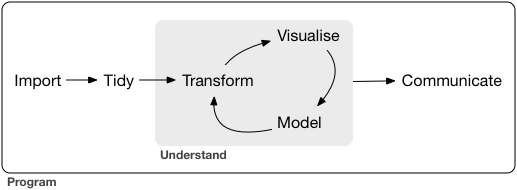
\includegraphics{https://d33wubrfki0l68.cloudfront.net/571b056757d68e6df81a3e3853f54d3c76ad6efc/32d37/diagrams/data-science.png}
\caption{Data science workflow from
\href{https://r4ds.had.co.nz}{\texttt{R} for Data Science}.}
\end{figure}


\end{document}
